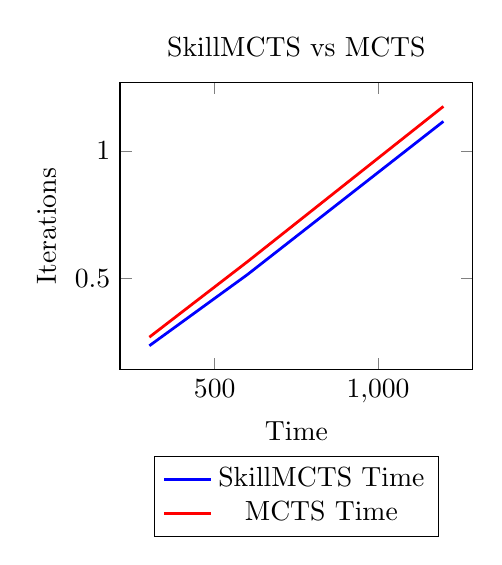
\begin{tikzpicture}
    \begin{axis}[
	    title={SkillMCTS vs MCTS},
	    width=0.5\linewidth,
	    xlabel = {Time},
        ylabel = {Iterations},
	    no marks, 
	    legend style={at={(0.5,-0.3)},anchor=north}
	    ]
        \addplot[line width=1pt, color=blue] coordinates {
           (300, 0.2379334)
           (600, 0.5162254)
           (1200, 1.1155539)
           };
        \addlegendentry{SkillMCTS Time}
        \addplot[line width=1pt, color=red] coordinates {
           (300, 0.2715728)
           (600, 0.5665983)
           (1200, 1.1741404)
           };
        \addlegendentry{MCTS Time}
    \end{axis}
\end{tikzpicture}